\documentclass{article}
\usepackage[utf8]{inputenc}
\usepackage{fullpage}
\usepackage{amsmath}
\usepackage{amsfonts}
\usepackage{amssymb}
\usepackage{amsthm}
\usepackage{algorithm}
\usepackage{algorithmicx}
\usepackage[noend]{algpseudocode}
\usepackage{multicol}
\usepackage{xspace}
\usepackage{stmaryrd}
\usepackage{graphicx}

\newtheorem{theorem}{Theorem}
\newtheorem{lemma}[theorem]{Lemma}
\newtheorem{definition}[theorem]{Definition}
\newtheorem{example}[theorem]{Example}

\newcommand{\var}[1]{\ensuremath{\textit{#1}}}
\newcommand{\interpret}[1]{\llbracket #1 \rrbracket}

\newcommand{\emptylist}{\ensuremath{[\:]}}

\newcommand{\lddnode}{\textsf{node}}
\newcommand{\lddright}{\textit{right}}
\newcommand{\ldddown}{\textit{down}}
\newcommand{\lddval}{\textit{val}}
\newcommand{\lddtrue}{\textsf{true}}
\newcommand{\lddfalse}{\textsf{false}} 

\title{List Decision Diagrams}
\author{Wieger Wesselink and Maurice Laveaux}
\date{\today}

\begin{document}

\newpage
\section{LD}

It can be compactly
represented using an LDD, see the figure below. For our applications we use the LDD implementation that is part of the Sylvan multi-core framework for decision diagrams, see
\cite{DBLP:journals/sttt/DijkP17}.

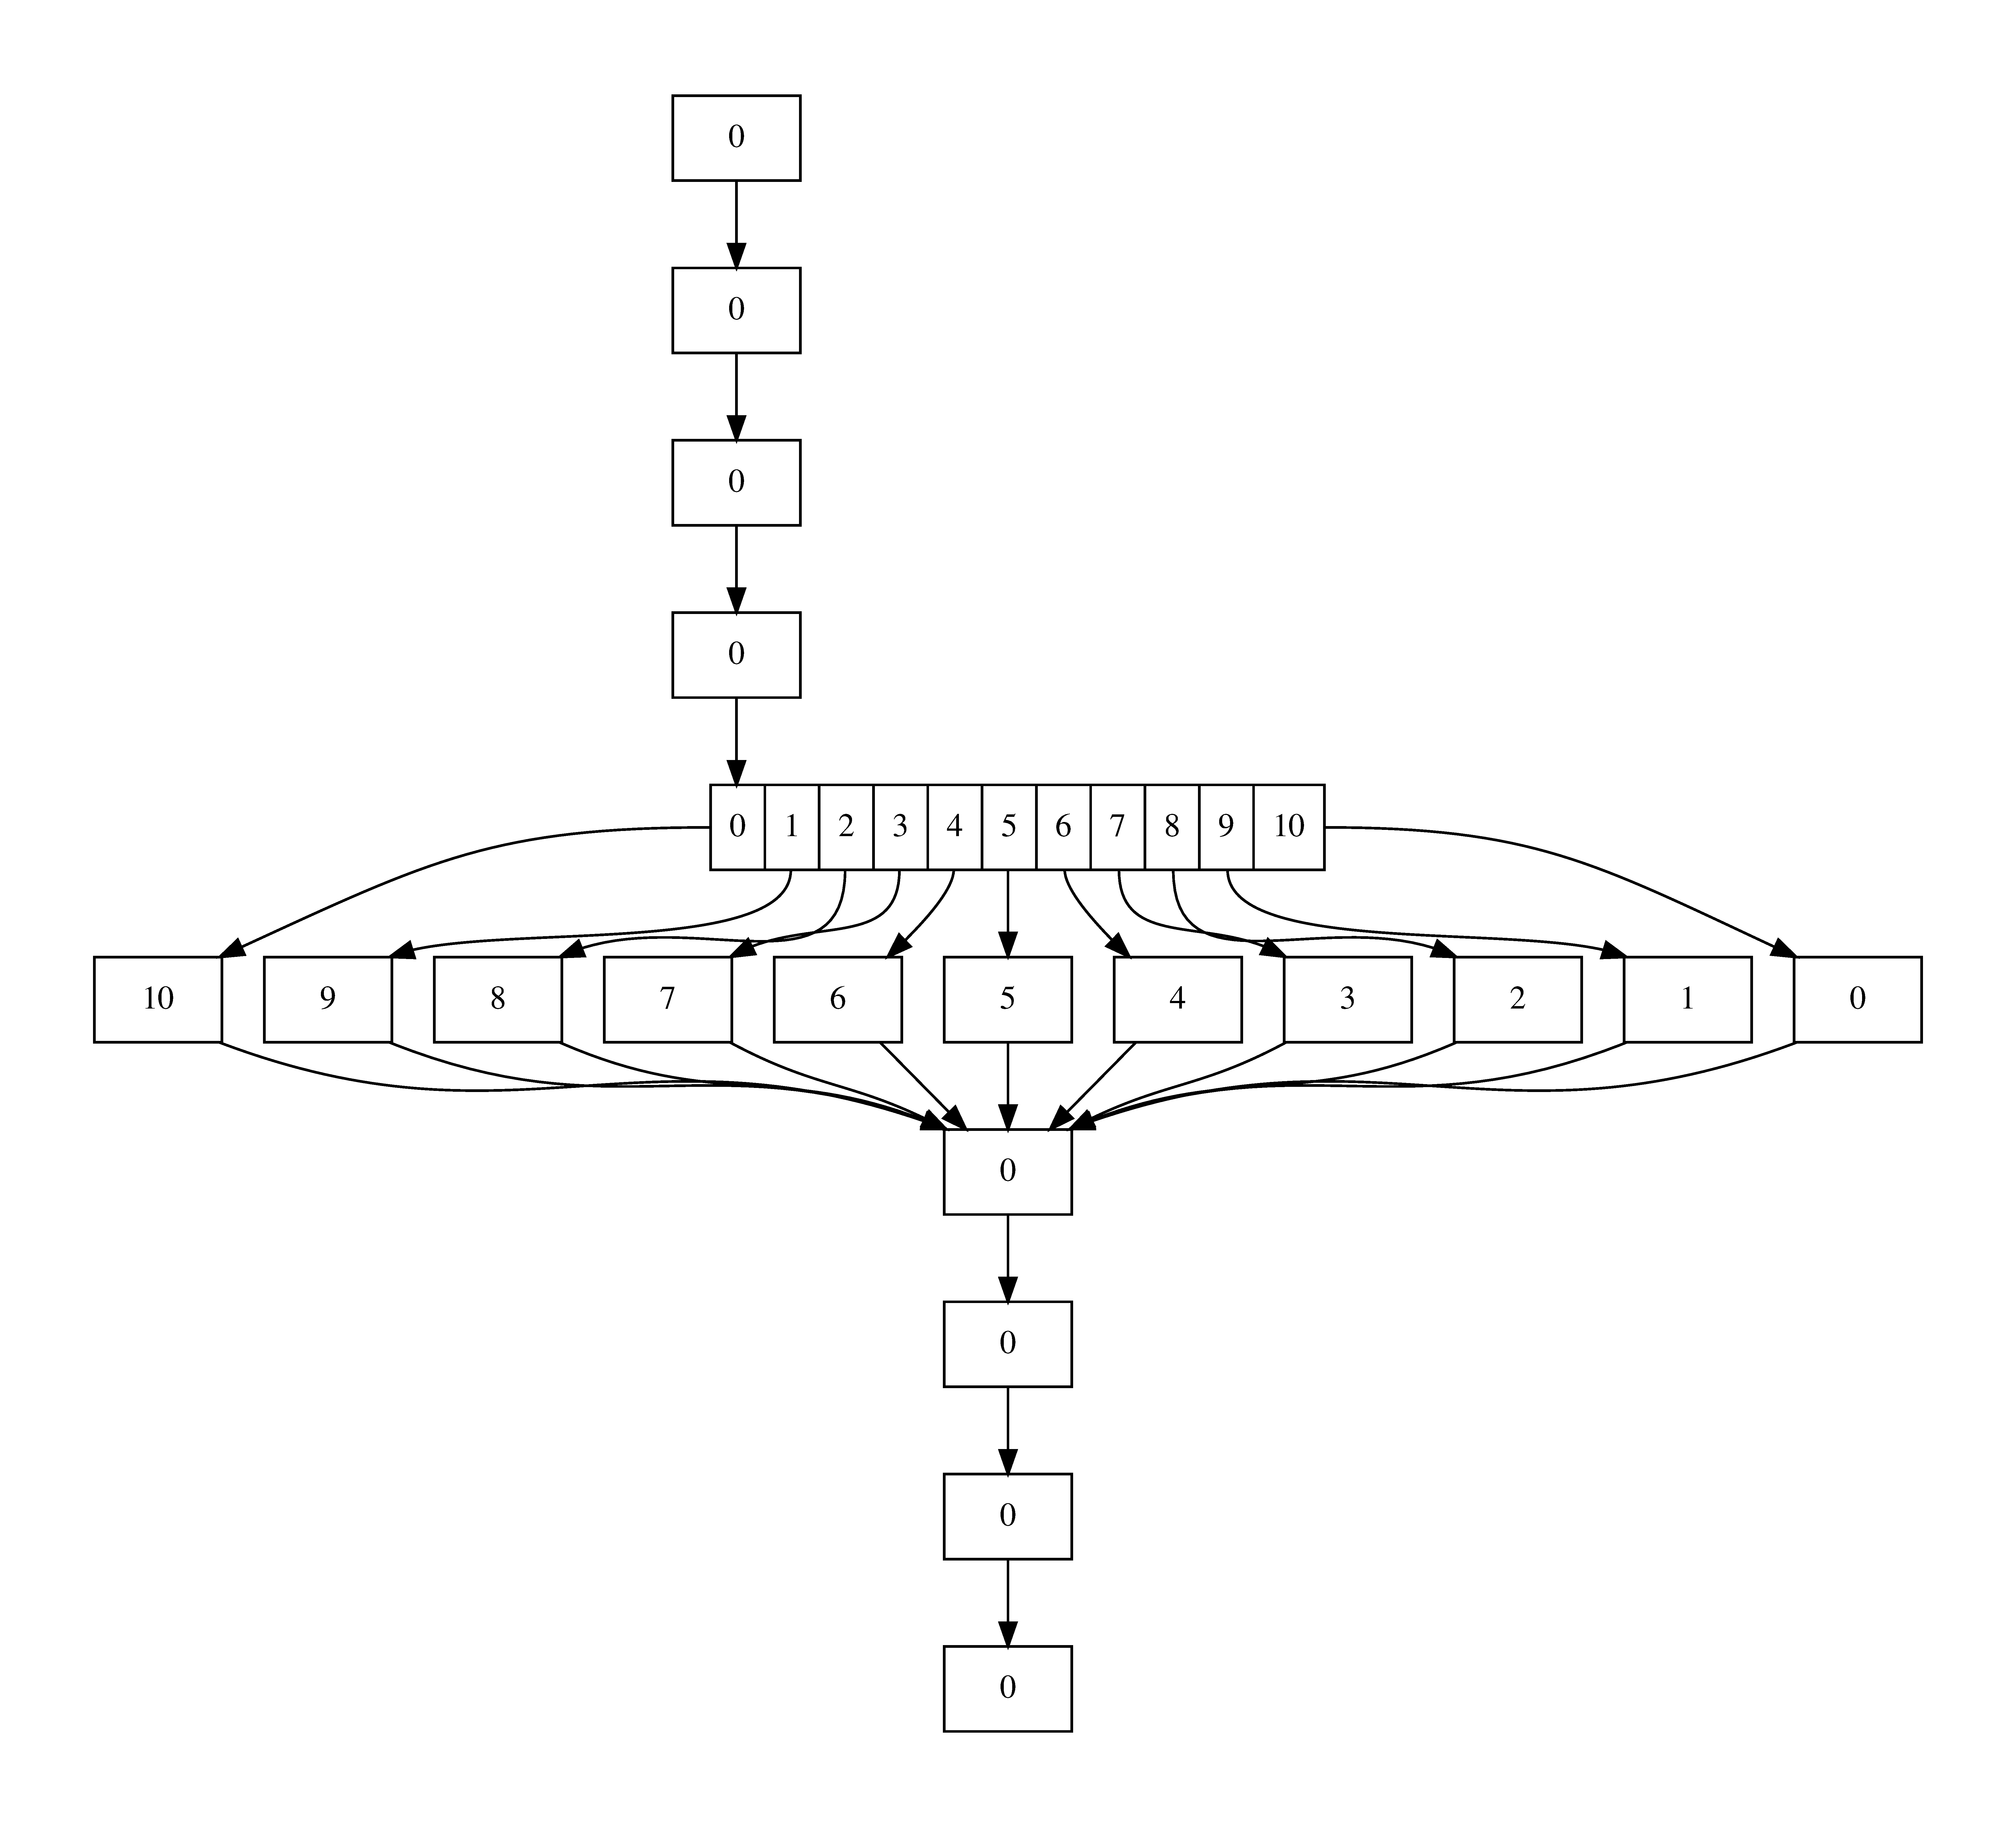
\includegraphics[width=15cm]{ldd_if_then.pdf}

For an LDD $A$ we use $\ldddown(A)$ to denote $A[x_i = v]$ and $\lddright(A)$ to denote $A[x_i > v]$.
We use $|A|$ to denote the size of the LDD, determined by the number of nodes.
Given a vector $v = x_0\,x_1 \cdots x_n$ we define its length, denoted by $|v|$, as $n + 1$.
Note that an LDD can represent (some) sets where two vectors have different lengths.
For example the set $\{1\,1, 0\}$ can be represented by an LDD.
However, the set $\{1\,1, 1\}$ cannot be represented since the root node can either have $\textsf{true}$ or $\var{node}(1, \textsf{true}, \textsf{false})$ as the down node and $\textsf{true}$ has no down or right nodes.
In general, we cannot represent a set with vectors that are strict prefixes (any vector $x_0 \cdots x_m$ with $m < n$ is a strict prefix of $v$) of other vectors in the set.
In practice, this means that we only consider LDDs where every vector in the represented set has the same length.
We refer to this length as the height of the LDD.
We often require that the input LDDs have equal height since not every output can be represented.
For example the union of $\{1\,1\}$ and $\{1\}$ cannot be represented as previously shown.

\subsection{Union}

We define the union operator on two equal height LDDs $A$ and $B$.
This computes the union of the represented sets of vectors.

\begin{algorithm}[h]
\caption{Union of two equal height LDDs $\var{A}$ and $\var{B}$}
\begin{algorithmic}[1]
\Function{union}{$A, B$}
\If{$A = B$}
	\State \Return $a$
\ElsIf{$A = \textsf{false}$}
	\State \Return $b$
\ElsIf{$B = \textsf{false}$}
	\State \Return $a$
\EndIf

\If{$val(A) < val(B)$}
	\State \Return $node(val(A), down(A), \textsc{union}(right(A), B))$
\ElsIf{$val(A) = val(B)$}
	\State \Return $node(val(A), \textsc{union}(down(A), down(B)), \textsc{union}(\lddright(A), right(B)))$
\ElsIf{$val(A) > val(B)$}
	\State \Return $node(val(B), down(B), \textsc{union}(A, right(B)))$	
\EndIf

\EndFunction
\end{algorithmic}
\end{algorithm}

\begin{lemma}
	For all LDDs $A$ and $B$ it holds that $\interpret{\textsc{union}(A, B)} = \interpret{A} \cup \interpret{B}$.
\end{lemma}
\begin{proof}
	Pick arbitrary LDDs $A$ and $B$.
	Proof by induction on the structure of $A$ and $B$.	
	For all LDDs $A'$ and $B'$ we assume that $\interpret{\textsc{union}(A', right(B'))} = \interpret{A'} \cup \interpret{right(B')}$ and $\interpret{\textsc{union}(A', down(B'))} = \interpret{A'} \cup \interpret{down(B')}$.
	Furthermore, $\interpret{\textsc{union}(\var{right}(A'), B')} = \interpret{\var{right}(A')} \cup \interpret{B'}$ and $\interpret{\textsc{union}(down(A'), B')} = \interpret{\var{down}(A')} \cup \interpret{B'}$.
	
	Base case.
	The LDD $A$ is either $\textsf{true}$ or $\textsf{false}$.
	Then $B$ is either $\textsf{true}$ or $\textsf{false}$ due to the equal height assumption.
	In both cases t he terminal conditions ensure correctness.
	For example $\interpret{\textsc{union}(\textsf{true}, \textsf{false})} = \interpret{\textsf{true}}$ and $\{[]\} \cup \emptyset = \{[]\}$.	
	Similarly, for the case where $B$ is either $\textsf{true}$ or $\textsf{false}$.
	
	Inductive step.
	\begin{itemize}
	\item Case $val(A) < val(B)$.
		Since $A$ is an LDD we know that $\lddval(A) < \lddval(\lddright(A))$.
		Therefore, we know that $\interpret{node(val(A), down(A), \textsc{union}(right(A), B))}$ is equal to $\{val(A)\,x \mid x \in \interpret{down(A)}\} \cup \interpret{\textsc{union}(right(A), B)}$.
		It follows that $\interpret{\textsc{union}(right(A), B)}$ is equal to $\interpret{right(A)} \cup \interpret{B}$.
		From which we can derive $\interpret{A} \cup \interpret{B}$.

	\item Case $val(A) = val(B)$.
		Since $A$ is an LDD we know that $\lddval(A) < \lddval(\lddright(A))$ and similarly because $B$ is an LDD we know that $\lddval(A) < \lddval(\lddright(B))$.
		Therefore, the following node is valid and $\interpret{node(val(A), \textsc{union}(down(A), down(B)), \textsc{union}(right(A), \var{right}(B)))}$ is equal to  $\{val(A)\,x \mid x \in \interpret{\textsc{union}(down(A), down(B))}\} \cup \interpret{\textsc{union}(right(A), right(B))}$.
		It follows that the interpretation $\{val(A)\,x \mid x \in \interpret{\textsc{union}(down(A), down(B))}$ is equal to $\{val(A)\,x \mid x \in \interpret{down(A)}\} \cup \{val(A)\,x \mid x \in \interpret{down(B)}\}$ and $\interpret{\textsc{union}(right(A), right(B))}$ is equal to $\interpret{(right(A)} \cup \interpret{right(B))}$.
%		From which we can derive $\interpret{right(A)} \cup \interpret{right(B)}$.
	
	\item Case $val(A) > val(B)$.
		Similar to the $val(A) < val(B)$ case.	\qedhere	
	\end{itemize} 
\end{proof}

We can show that $|\textsc{union(A, B)}|$ for any LDDs $A$ and $B$ is at most $|A| + |B|$.
The time complexity of $\textsc{union(A, B)}$ is also of order $\mathcal{O}(|A| + |B|)$.

\subsection{Project}

Given a vector $x_0\,\cdots\,x_n$ and a subset $I \subseteq \mathbb{N}$, we define the \emph{projection}, denoted by $\textit{project}(x_0\,\cdots\,x_n, I)$, as the vector $x_{i_0}, \ldots, x_{i_l}$ for the largest $l \in \mathbb{N}$ such that $i_0 < i_1 < \ldots < i_l \leq n$ and $i_k \in I$ for $0 \leq k \leq l$.
We define the projection operator for an LDD where every vector in the set is projected.
For the LDD operator it is more convenient to specify the indices $I \subseteq \mathbb{N}$ by a vector $x_0\,\cdots\,x_n$ such that for $0 \leq i \leq n$ variable $x_i$ is one iff $i \in I$.
The operator takes an LDD $A$ of height $n$ and a sequence of numbers $x_0\,x_1,\cdots\,x_n$.

\begin{algorithm}[h]
\caption{Project vectors of an LDD $\var{A}$ of height $n$ using a sequence $x_0\,\cdots\,x_n$}
\begin{algorithmic}[1]
\Function{project}{$A, x_0\,x_1\,\cdots\,x_n$}
	\If{$A = \lddtrue$}
		\State \Return $\lddtrue$
	\ElsIf{$A = \lddfalse$}
		\State \Return $\lddfalse$
	\EndIf
	
	\If{$x_0 = 1$}
		\State \Return{$\lddnode(\lddval(A), \textsc{project}(\ldddown(A), x_1\,\cdots\,x_n), \textsc{project}(\lddright(A), x_0\,\cdots\,x_n))$}
	\ElsIf{$x_0 = 0$}
		\State $a \gets A$
		\State $R \gets \lddfalse$
		\While {$a \neq \lddfalse$}
			\State $R \gets \textsc{union}(R, \textsc{project}(\ldddown(a), x_1\,\cdots\,x_n))$
			\State $a \gets \lddright(a)$		
		\EndWhile			
		\State \Return {$R$}
	\EndIf

\EndFunction
\end{algorithmic}
\end{algorithm}

\begin{lemma}
	For all LDDs $A$ and sequences $x_0\,x_1\,\cdots\,x_n $it holds that $\interpret{\textsc{project}(A, x_0\,\cdots\,x_n)}$ is equal to $\{\textit{project}(v, x_0\,\cdots\,x_n) \in \interpret{A}\}$.
\end{lemma}

Note that for a sequence of $|A|$ zeroes $\textsc{project}(A, 0\,\cdots\,0)$ is equal to $\lddtrue$ and for a sequence of $|A|$ ones $\textsc{project}(A, 1\,\cdots\,1)$ is equal to $A$.

\subsection{Caching}

We can speed up LDD operations at the cost of memory by using an operation cache.
For every operation there will be a separate \emph{global} cache, represented by a set, that stores a tuple of the inputs and the output.
We use \emph{global} to emphasize that every recursion sees the latest values stored in the cache.  
For example the $\textsc{union}(A, B)$ operation has a cache $C_\textsc{union}$ and the pseudocode of $\textsc{union}$ is changed such that after the terminal cases first we check whether $\exists R : (A, B, R) \in C_\textsc{union}$ and return the result $R$ if that is the case.
Otherwise, we perform the computation as before but store the result in $C_\textsc{union}$ instead before returning it.
Thus we obtain the following algorithm:

\begin{algorithm}[H]
\caption{Union of two LDDs $\var{A}$ and $\var{B}$.
	With a set $C_\textsc{union}$ as operation cache}
\begin{algorithmic}[1]
\Function{union}{$A, B,  C_\textsc{union}$}
\If{$A = B$}
	\State \Return $a$
\ElsIf{$A = \textsf{false}$}
	\State \Return $b$
\ElsIf{$B = \textsf{false}$}
	\State \Return $a$
\EndIf

\If{$\exists R: (A, B, R) \in C_\textsc{union}$}
	\Return $R$
\EndIf

\If{$val(A) < val(B)$}
	\State $R \gets node(val(A), down(A), \textsc{union}(right(A), B, C_\textsc{union}))$
\ElsIf{$val(A) = val(B)$}
	\State $R \gets node(val(A), union(down(A), down(B), union(right(A), right(B), C_\textsc{union}))$
\ElsIf{$val(A) > val(B)$}
	\State $R \gets node(val(B), down(B), \textsc{union}(A, right(B), C_\textsc{union}))$
\EndIf

\State $C_\textsc{union} \gets C_\textsc{union} \cup \{(A, B, R)\}$
\State \Return $R$
\EndFunction
\end{algorithmic}
\end{algorithm}

\subsection{Parallelism}

In some cases we can improve the performance further by computing several results in parallel during the operation.
For example in the union of two LDDs $A$ and $B$ in the case $val(A) = val(B)$ we could determine the result of both unions in parallel and only merge them after they have finished.

\bibliographystyle{plain}
\bibliography{symbolic-reachability}
\end{document}
